\documentclass[11pt,letterpaper]{article}
\usepackage[margin=0.9in]{geometry}
\usepackage[T1]{fontenc}
\usepackage{lmodern}
\usepackage{microtype}
\usepackage{siunitx}
\usepackage{booktabs}
\usepackage{tabularx}
\usepackage{array}
\usepackage{xcolor}
\usepackage{tikz}
\usetikzlibrary{arrows.meta,calc,positioning,decorations.pathreplacing,patterns}
\usepackage[siunitx]{circuitikz}
\usepackage[colorlinks=true,linkcolor=blue!50!black,urlcolor=blue!50!black]{hyperref}
\usepackage{enumitem}
\usepackage[section]{placeins}
\setlist{nosep,leftmargin=*}

\sisetup{per-mode=symbol}
\newcommand{\id}[1]{\textsf{\textbf{#1}}}  % inventory ID, as used in the figures

\title{Front-yard holiday LED display\\[2pt]\large Design: frame, W-modules, power fan-out}
\author{henderson (with Michael Mulhearn)}
\date{2026-10-19, phase~1}

\begin{document}
\maketitle

\noindent Inventory IDs in \id{bold sans} (e.g.\ \id{LED-1}) refer to the bill of materials in
Section~\ref{sec:bom} and appear in the figures.  The controller (Trenz Zynq module and level shifter) is
described separately; this document stops at the data input of the first module.

\section{Overview}

\begin{itemize}
  \item \textbf{Panel:} $56 \times 37$ square pixels at \SI{33.3}{mm} (\SI{1.31}{in}) pitch, the pitch of a
    30-LED/m strip, both across and down: an LED area of $\SI{73.5}{in} \times \SI{48.6}{in}$, 2072 pixels.
  \item \textbf{Strip:} WS2815, \SI{12}{V}, 30~LEDs/m, IP65 (\id{LED-1}); every LED individually addressable,
    with a backup data line (a dead LED does not darken the rest of the chain).
  \item \textbf{Modules:} 14 identical four-column \emph{W-modules}, one \SI{5}{m} reel each (148 of its 150
    LEDs), plus one spare reel.
  \item \textbf{Power:} one sealed Mean Well HLG-600H-12B (\id{PS-1}, \SI{12}{V} \SI{40}{A} \SI{480}{W}, IP67);
    one \SI{5}{A} fuse and one 18~AWG home run per module.
  \item \textbf{Brightness cap:} 50\,\% in software (WLED or our own); up to about 75\,\% stays comfortable for
    the supply (Section~\ref{sec:numbers}).
  \item \textbf{Phase 1} is the full panel.  A pilot (one module, Section~\ref{sec:pilot}) comes first.
\end{itemize}

\section{Frame}

The frame is a box of 2x6 on edge (\id{FR-1}), sized to the LED area plus clearance, with a 2x4 rail
standing up across the inside at top and bottom (\id{FR-2}) and one 1x2 slat (\id{FR-3}) per two columns,
screwed to the front of both rails (Figures~\ref{fig:frame-front} and~\ref{fig:frame-section}).
\begin{itemize}
  \item \textbf{Outside} about $\SI{77}{in} \times \SI{59}{in} \times \SI{5.5}{in}$; inside
    $\SI{74}{in} \times \SI{56}{in}$.  Lumber: 8~ft boards only, scrap used elsewhere.
  \item \textbf{Rails} (\id{FR-2}): 2x4 standing up (\SI{3.5}{in} high, \SI{1.5}{in} deep), set back from the
    front so that slat, strip and an optional diffuser fit within the box depth.  The top rail area carries
    the connections; the bottom rail only holds the slats.
  \item \textbf{Slats} (\id{FR-3}): 28 1x2 ($\SI{0.75}{in} \times \SI{1.5}{in}$), each about \SI{56}{in} long,
    at a pitch of two columns (\SI{66.7}{mm}); each carries two columns \SI{33.3}{mm} apart, centered.  The
    \SI{10}{mm} strips overhang the \SI{38}{mm} slat by about \SI{3}{mm} each side, which is fine.  A spacing jig
    on the rails keeps the pitch; gaps of about \SI{29}{mm} leave the panel about 40\,\% open to wind and air.
  \item \textbf{Clips} (\id{MNT-1}): three per column (top, middle, bottom), screwed to the slat; 12~mm clips for
    the 10~mm strip in its IP65 coat.
  \item \textbf{Weather:} a rain cover with a drip edge over the top; all connections in the top rail area,
    under it.  The supply (\id{PS-1}) is sealed and mounts on a backing plate behind the top rail; the fuse
    blocks and bus bars sit in a covered box beside it (\id{HD-5}).
  \item \textbf{Mounting:} on the low masonry wall in front of the house: a shoe over the wall cap, ropes from
    the top corners to the eaves (against falling forward), struts behind (against falling back); lay it flat
    in storms.
  \item \textbf{Measure first:} the frame's dimensions assume a \SI{33.3}{mm} pitch.  Measure the pilot reel
    over 37 LEDs before cutting the 2x6.
\end{itemize}

\begin{figure}[!htbp]
  \centering
  % Frame, front elevation, to scale (units: inches).
% Outside 77 x 59; 2x6 (1.5 thick); rails 2x4 standing up (3.5 high); 28 slats 1x2 (1.5 wide) at 2 columns
% (2 x 1.3123 in) pitch; LED area 56 x 37 at 1.3123 in pitch = 73.49 x 48.56, centered in the 74 x 56 inside.
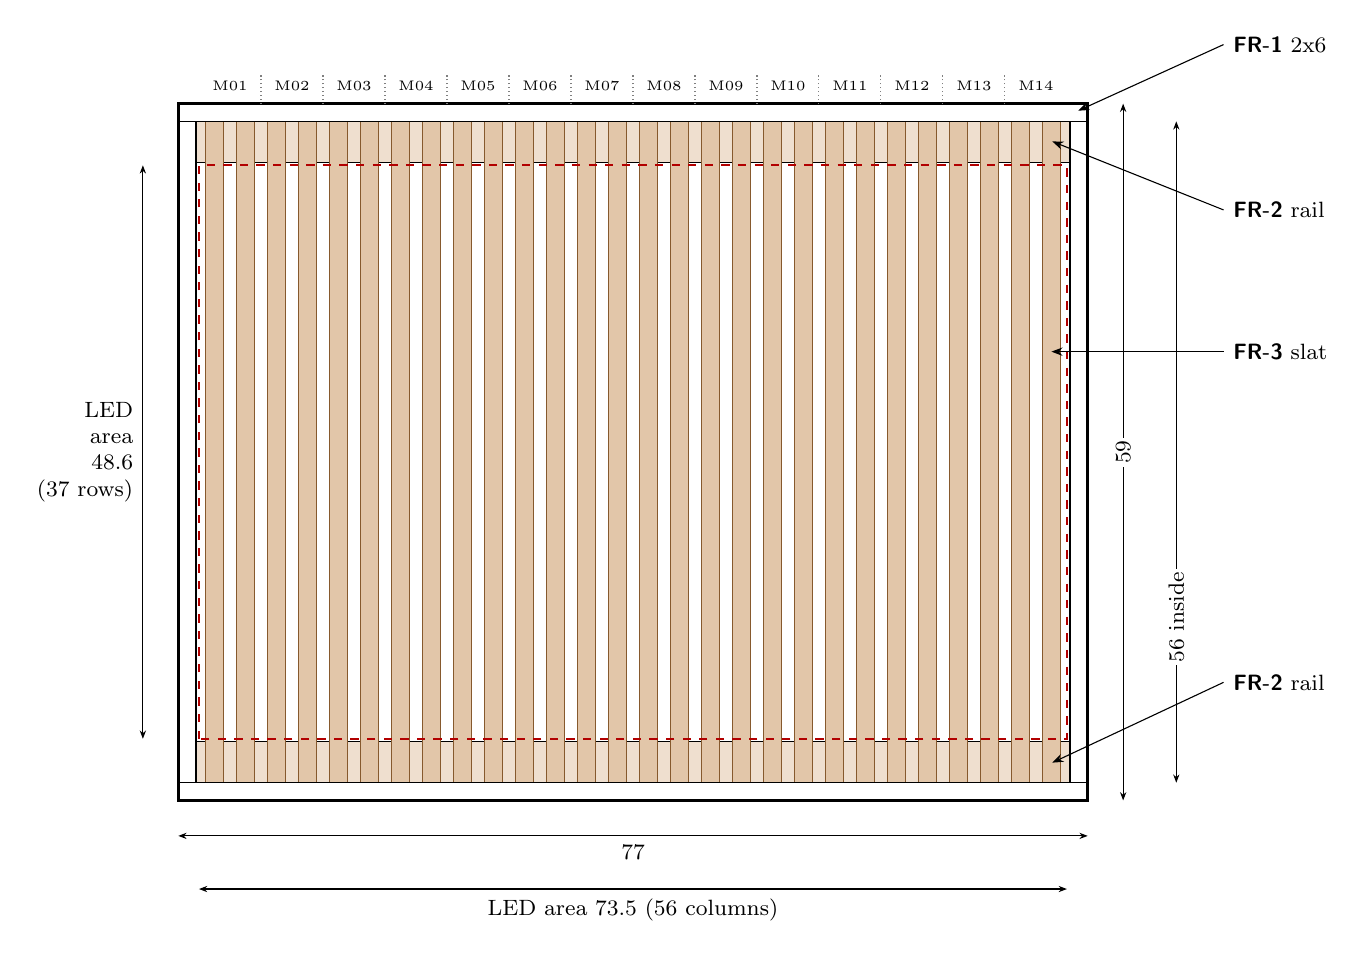
\begin{tikzpicture}[x=0.15cm,y=0.15cm, font=\footnotesize,
    callout/.style={-{Stealth[length=4pt]}, thin},
    dim/.style={{Stealth[length=3pt]}-{Stealth[length=3pt]}, thin}]
  \def\p{1.3123}      % column pitch, inches
  \def\xl{1.75}       % LED area left edge
  \def\yb{5.22}       % LED area bottom
  \def\yt{53.78}      % LED area top
  % rails (behind the slats)
  \fill[brown!25] (1.5,1.5) rectangle (75.5,5.0);
  \fill[brown!25] (1.5,54.0) rectangle (75.5,57.5);
  \draw (1.5,1.5) rectangle (75.5,5.0);
  \draw (1.5,54.0) rectangle (75.5,57.5);
  % slats
  \foreach \s in {0,...,27} {
    \pgfmathsetmacro{\xc}{\xl + (2*\s+1)*\p}
    \fill[brown!45] (\xc-0.75,1.5) rectangle (\xc+0.75,57.5);
    \draw[brown!70!black] (\xc-0.75,1.5) rectangle (\xc+0.75,57.5);
  }
  % 2x6 box
  \draw[very thick] (0,0) rectangle (77,59);
  \draw (1.5,1.5) rectangle (75.5,57.5);
  \draw (0,1.5) -- (1.5,1.5) (75.5,1.5) -- (77,1.5) (0,57.5) -- (1.5,57.5) (75.5,57.5) -- (77,57.5);
  % LED area
  \draw[dashed, red!70!black, thick] (\xl,\yb) rectangle (\xl+56*\p,\yt);
  % module labels and boundaries
  \foreach \k in {0,...,13} {
    \pgfmathsetmacro{\xm}{\xl + (4*\k+2)*\p}
    \pgfmathtruncatemacro{\n}{\k+1}
    \node[font=\tiny, above] at (\xm,59.3) {M\ifnum\n<10 0\fi\n};
  }
  \foreach \k in {1,...,13} {
    \pgfmathsetmacro{\xb}{\xl + 4*\k*\p}
    \draw[densely dotted, gray] (\xb,59) -- (\xb,61.5);
  }
  % dimensions
  \draw[dim] (0,-3) -- node[below] {77} (77,-3);
  \draw[dim] (\xl,-7.5) -- node[below] {LED area 73.5 (56 columns)} (\xl+56*\p,-7.5);
  \draw[dim] (80,0) -- node[midway, fill=white, inner sep=1pt, rotate=90] {59} (80,59);
  \draw[dim] (-3,\yb) -- node[left, align=right] {LED\\area\\48.6\\(37 rows)} (-3,\yt);
  \draw[dim] (84.5,1.5) -- node[pos=0.25, fill=white, inner sep=1pt, rotate=90] {56 inside} (84.5,57.5);
  % callouts
  \draw[callout] (88.5,64) node[right] {\id{FR-1} 2x6} -- (76.2,58.4);
  \draw[callout] (88.5,50) node[right] {\id{FR-2} rail} -- (74,55.8);
  \draw[callout] (88.5,10) node[right] {\id{FR-2} rail} -- (74,3.2);
  \draw[callout] (88.5,38) node[right] {\id{FR-3} slat} -- (\xl+55*\p,38);
\end{tikzpicture}

  \caption{Frame, front elevation (to scale).  2x6 box \id{FR-1}, rails \id{FR-2}, 28 slats \id{FR-3} (two per
    module, M01--M14), LED area dashed.  Dimensions in inches.}
  \label{fig:frame-front}
\end{figure}

\begin{figure}[!htbp]
  \centering
  % Frame, vertical section through a slat (side view), not to scale vertically; depths in inches.
% Front (viewer) on the left.  Proposed depths: diffuser at the front plane, ~1.25 air gap, strip ~0.15,
% slat 0.75, rail 1.5 deep (3.5 high), wiring space behind to the 5.5 box depth.
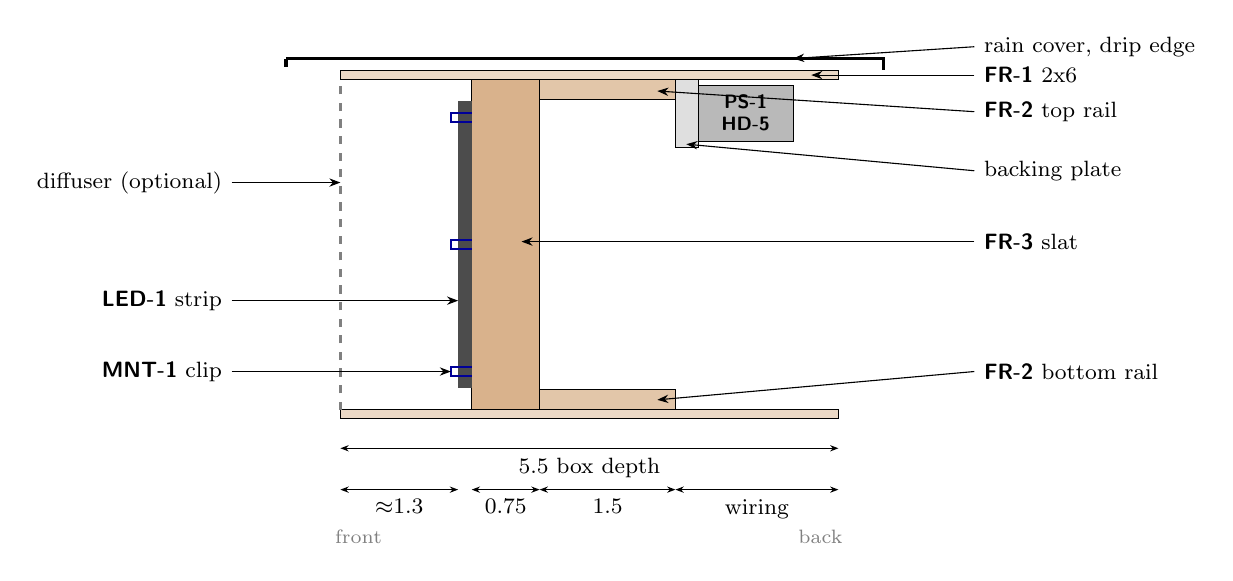
\begin{tikzpicture}[x=1.15cm,y=0.075cm, font=\footnotesize,
    callout/.style={-{Stealth[length=4pt]}, thin},
    dim/.style={{Stealth[length=3pt]}-{Stealth[length=3pt]}, thin}]
  % box sides (top and bottom 2x6, seen in section): depth 0..5.5, 1.5 thick
  \fill[brown!30] (0,57.5) rectangle (5.5,59);
  \fill[brown!30] (0,0) rectangle (5.5,1.5);
  \draw (0,57.5) rectangle (5.5,59);
  \draw (0,0) rectangle (5.5,1.5);
  % rails: depth 2.2..3.7, heights 1.5..5.0 and 54.0..57.5
  \fill[brown!45] (2.2,54.0) rectangle (3.7,57.5);
  \fill[brown!45] (2.2,1.5) rectangle (3.7,5.0);
  \draw (2.2,54.0) rectangle (3.7,57.5);
  \draw (2.2,1.5) rectangle (3.7,5.0);
  % slat: depth 1.45..2.2, full height 1.5..57.5
  \fill[brown!60] (1.45,1.5) rectangle (2.2,57.5);
  \draw (1.45,1.5) rectangle (2.2,57.5);
  % strip on the slat front: depth 1.3..1.45, LED area 5.22..53.78
  \fill[black!70] (1.3,5.22) rectangle (1.45,53.78);
  % clips (top, middle, bottom)
  \foreach \y in {8,29.5,51} { \draw[thick, blue!60!black] (1.45,\y-0.8) -- (1.22,\y-0.8) -- (1.22,\y+0.8) -- (1.45,\y+0.8); }
  % diffuser (optional) at the front plane
  \draw[dashed, thick, gray] (0,1.5) -- (0,57.5);
  % supply and covered box behind the top rail (backing plate)
  \fill[gray!25] (3.7,46) rectangle (3.95,57.5);
  \draw (3.7,46) rectangle (3.95,57.5);
  \fill[gray!55] (3.95,47) rectangle (5.0,56.5);
  \draw (3.95,47) rectangle (5.0,56.5) node[midway, font=\scriptsize, align=center] {\id{PS-1}\\\id{HD-5}};
  % rain cover
  \draw[very thick] (-0.6,61) -- (6.0,61) -- (6.0,59);
  \draw[very thick] (-0.6,61) -- (-0.6,59.5);
  % labels
  \draw[callout] (-1.2,40) node[left] {diffuser (optional)} -- (0,40);
  \draw[callout] (-1.2,20) node[left] {\id{LED-1} strip} -- (1.3,20);
  \draw[callout] (-1.2,8) node[left] {\id{MNT-1} clip} -- (1.22,8);
  \draw[callout] (7.0,30) node[right] {\id{FR-3} slat} -- (2.0,30);
  \draw[callout] (7.0,52) node[right] {\id{FR-2} top rail} -- (3.5,55.5);
  \draw[callout] (7.0,8) node[right] {\id{FR-2} bottom rail} -- (3.5,3.2);
  \draw[callout] (7.0,58.2) node[right] {\id{FR-1} 2x6} -- (5.2,58.2);
  \draw[callout] (7.0,63) node[right] {rain cover, drip edge} -- (5.0,61);
  \draw[callout] (7.0,42) node[right] {backing plate} -- (3.82,46.5);
  % depth dimensions
  \draw[dim] (0,-5) -- node[below] {5.5 box depth} (5.5,-5);
  \draw[dim] (0,-12) -- node[below] {$\approx$1.3} (1.3,-12);
  \draw[dim] (1.45,-12) -- node[below] {0.75} (2.2,-12);
  \draw[dim] (2.2,-12) -- node[below] {1.5} (3.7,-12);
  \draw[dim] (3.7,-12) -- node[below] {wiring} (5.5,-12);
  \node[font=\scriptsize, gray] at (0.2,-20) {front};
  \node[font=\scriptsize, gray] at (5.3,-20) {back};
\end{tikzpicture}

  \caption{Frame, vertical section through a slat (not to scale; depths in inches, proposed).  From the front:
    optional diffuser, air gap, strip \id{LED-1} in its clip \id{MNT-1}, slat \id{FR-3}, rail \id{FR-2}, then
    space for wiring behind.  The supply \id{PS-1} and the covered box \id{HD-5} sit behind the top rail.}
  \label{fig:frame-section}
\end{figure}

\section{W-module}

Each module is one reel (\id{LED-1}) folded into four columns of 37 LEDs (Figure~\ref{fig:w-module}):
\begin{itemize}
  \item \textbf{Path:} the data enters at the top of column~1 and runs down; corner C1 (bottom) turns it up
    column~2; corner C2 (top) down column~3; corner C3 (bottom) up column~4; it leaves at the top of
    column~4.  Input and output are both at the top, \SI{100}{mm} apart.
  \item \textbf{Spare LEDs:} $4 \times 37 = 148$ of 150.  The two spare LEDs are cut out at corner C1, so both
    factory ends, with their 4-pin plugs, stay on the module.
  \item \textbf{Corners:} each corner is cut at the strip's cut marks and joined by four short 18~AWG jumpers
    (\id{WIR-1}): \SI{12}{V}, data (DO to DI), backup data (BO to BI) and ground (Figure~\ref{fig:corner}).
    Each cut end is sealed with \SI{1.25}{in} of adhesive-lined 1/2'' heat shrink (\id{HS-1}): six per module.
  \item \textbf{Electrically} the module behaves as one uncut reel; the jumpers carry current better than the
    strip's own copper.
  \item \textbf{Power:} fed at the input end only, through the input plug's power leads (12~V constant-current
    LEDs tolerate the drop along the strip; checked on the pilot, and the far-end ``voltage compensation''
    pigtail is in reserve).
  \item \textbf{Data:} modules plug together: module $k$'s output plug into module $k{+}1$'s input plug.  The
    first module's backup input BI is tied to ground.
  \item \textbf{Mounting:} the two slats of a module are its carrier; a module comes off with its clips.
\end{itemize}

\begin{figure}[!htbp]
  \centering
  % W-module: four columns of 37 on two slats, data path, corners C1-C3, plugs.  Schematic: only some LEDs drawn
% (the first and last 5 of each column), vertical scale compressed.
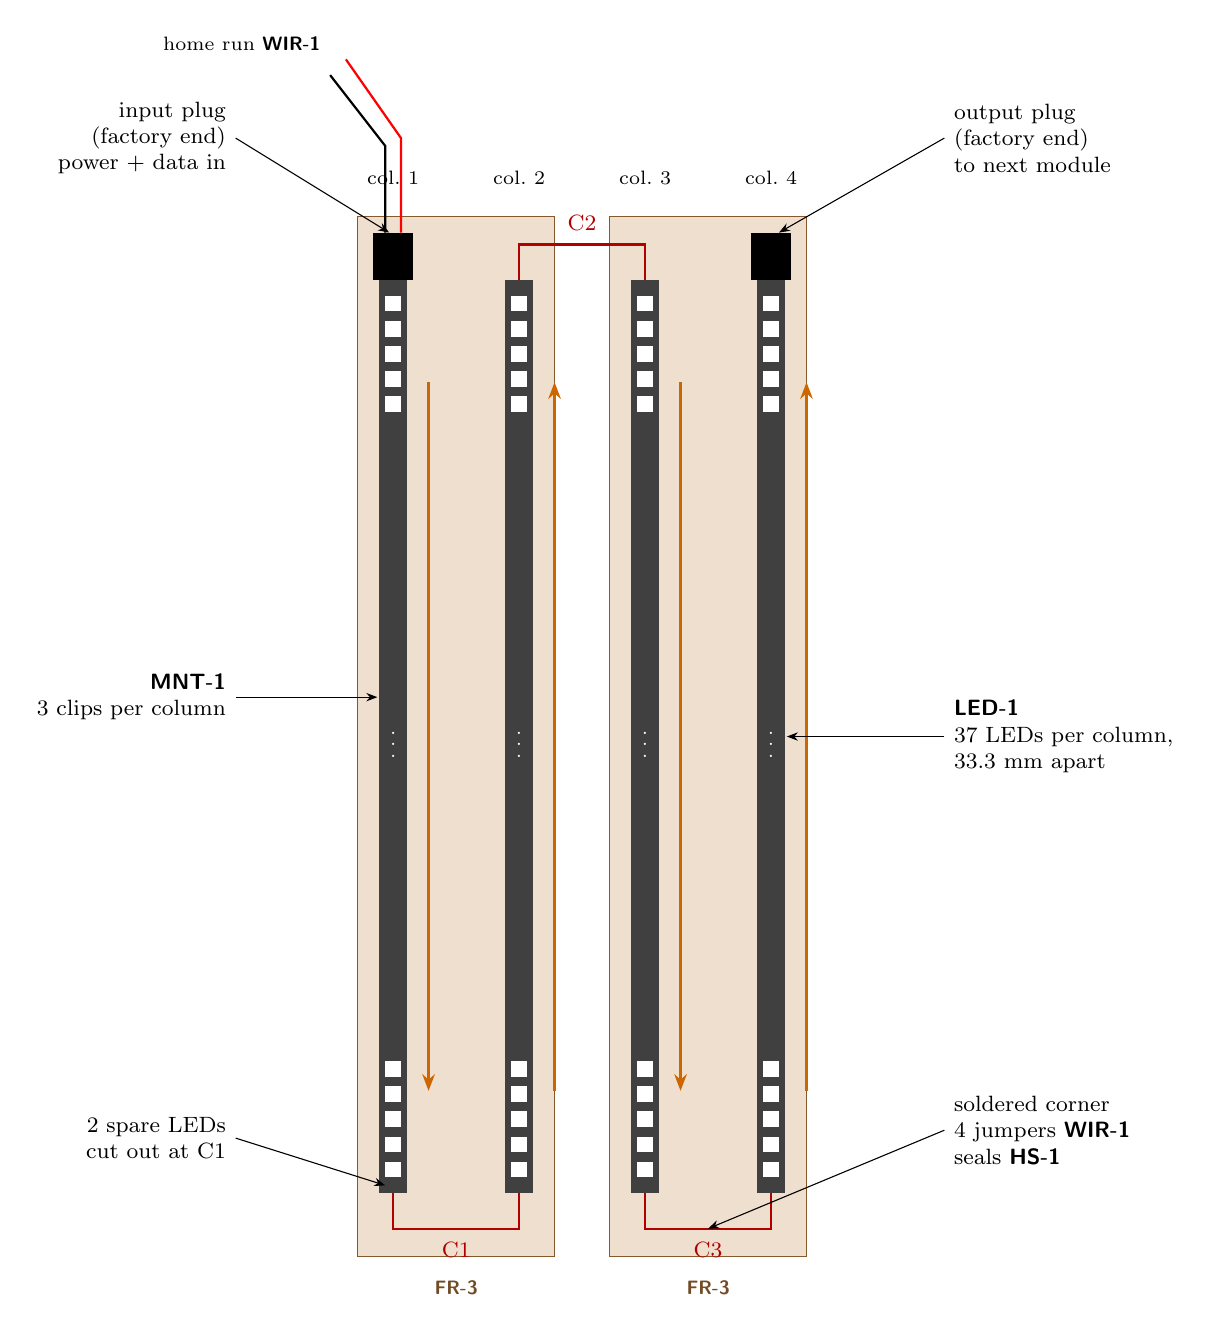
\begin{tikzpicture}[font=\footnotesize,
    callout/.style={-{Stealth[length=4pt]}, thin},
    flow/.style={-{Stealth[length=6pt]}, very thick, orange!80!black}]
  \def\dx{1.6}   % column spacing (drawing units, cm)
  \def\dy{0.32}  % LED spacing
  % slats: two, each under two columns
  \foreach \s in {0,1} {
    \pgfmathsetmacro{\xc}{(2*\s+0.5)*\dx}
    \fill[brown!25] (\xc-1.25,-0.6) rectangle (\xc+1.25,12.6);
    \draw[brown!70!black] (\xc-1.25,-0.6) rectangle (\xc+1.25,12.6);
  }
  \node[brown!60!black, font=\scriptsize] at (0.5*\dx,-1.0) {\id{FR-3}};
  \node[brown!60!black, font=\scriptsize] at (2.5*\dx,-1.0) {\id{FR-3}};
  % columns of LEDs (strip body + LEDs: top 5 and bottom 5 drawn, dots in between)
  \foreach \c in {0,...,3} {
    \pgfmathsetmacro{\x}{\c*\dx}
    \fill[black!75] (\x-0.18,0.2) rectangle (\x+0.18,11.8);
    \foreach \i in {0,...,4} {
      \fill[white] (\x-0.1,11.5-\i*\dy-0.1) rectangle (\x+0.1,11.5-\i*\dy+0.1);
      \fill[white] (\x-0.1,0.5+\i*\dy-0.1) rectangle (\x+0.1,0.5+\i*\dy+0.1);
    }
    \node[white, font=\scriptsize] at (\x,6) {$\vdots$};
    \node[font=\scriptsize] at (\x,13.1) {col.~\the\numexpr\c+1\relax};
  }
  % data flow arrows along each column
  \draw[flow] (0.45,10.5) -- (0.45,1.5);
  \draw[flow] (\dx+0.45,1.5) -- (\dx+0.45,10.5);
  \draw[flow] (2*\dx+0.45,10.5) -- (2*\dx+0.45,1.5);
  \draw[flow] (3*\dx+0.45,1.5) -- (3*\dx+0.45,10.5);
  % corners
  \draw[thick, red!70!black] (0,0.2) -- (0,-0.25) -- (\dx,-0.25) -- (\dx,0.2);
  \draw[thick, red!70!black] (\dx,11.8) -- (\dx,12.25) -- (2*\dx,12.25) -- (2*\dx,11.8);
  \draw[thick, red!70!black] (2*\dx,0.2) -- (2*\dx,-0.25) -- (3*\dx,-0.25) -- (3*\dx,0.2);
  \node[red!70!black, below] at (0.5*\dx,-0.3) {C1};
  \node[red!70!black, above] at (1.5*\dx,12.3) {C2};
  \node[red!70!black, below] at (2.5*\dx,-0.3) {C3};
  % plugs
  \fill[black] (-0.25,11.8) rectangle (0.25,12.4);
  \fill[black] (3*\dx-0.25,11.8) rectangle (3*\dx+0.25,12.4);
  % callouts
  \draw[callout] (-2.0,13.6) node[left, align=right] {input plug\\(factory end)\\power + data in} -- (-0.05,12.4);
  \draw[callout] (3*\dx+2.2,13.6) node[right, align=left] {output plug\\(factory end)\\to next module} -- (3*\dx+0.1,12.4);
  \draw[callout] (-2.0,0.9) node[left, align=right] {2 spare LEDs\\cut out at C1} -- (-0.1,0.3);
  \draw[callout] (3*\dx+2.2,6) node[right, align=left] {\id{LED-1}\\37 LEDs per column,\\33.3~mm apart} -- (3*\dx+0.2,6);
  \draw[callout] (3*\dx+2.2,1.0) node[right, align=left] {soldered corner\\4 jumpers \id{WIR-1}\\seals \id{HS-1}} -- (2.5*\dx,-0.25);
  \draw[callout] (-2.0,6.5) node[left, align=right] {\id{MNT-1}\\3 clips per column} -- (-0.2,6.5);
  % home run arrives at the input plug
  \draw[thick, red] (0.1,12.4) -- (0.1,13.6) -- (-0.6,14.6);
  \draw[thick, black] (-0.1,12.4) -- (-0.1,13.5) -- (-0.8,14.4);
  \node[font=\scriptsize, align=right, left] at (-0.8,14.8) {home run \id{WIR-1}};
\end{tikzpicture}

  \caption{W-module: one reel \id{LED-1} as four columns of 37 on two slats \id{FR-3} (LEDs not all drawn).
    Arrows: data direction.  C1--C3: soldered corners (Figure~\ref{fig:corner}); the two spare LEDs are cut out
    at C1.  Input and output are the reel's factory plugs; power enters at the input.}
  \label{fig:w-module}
\end{figure}

\begin{figure}[!htbp]
  \centering
  % Corner joint detail: two strip ends (cut), four 18 AWG jumpers, heat-shrink seals.
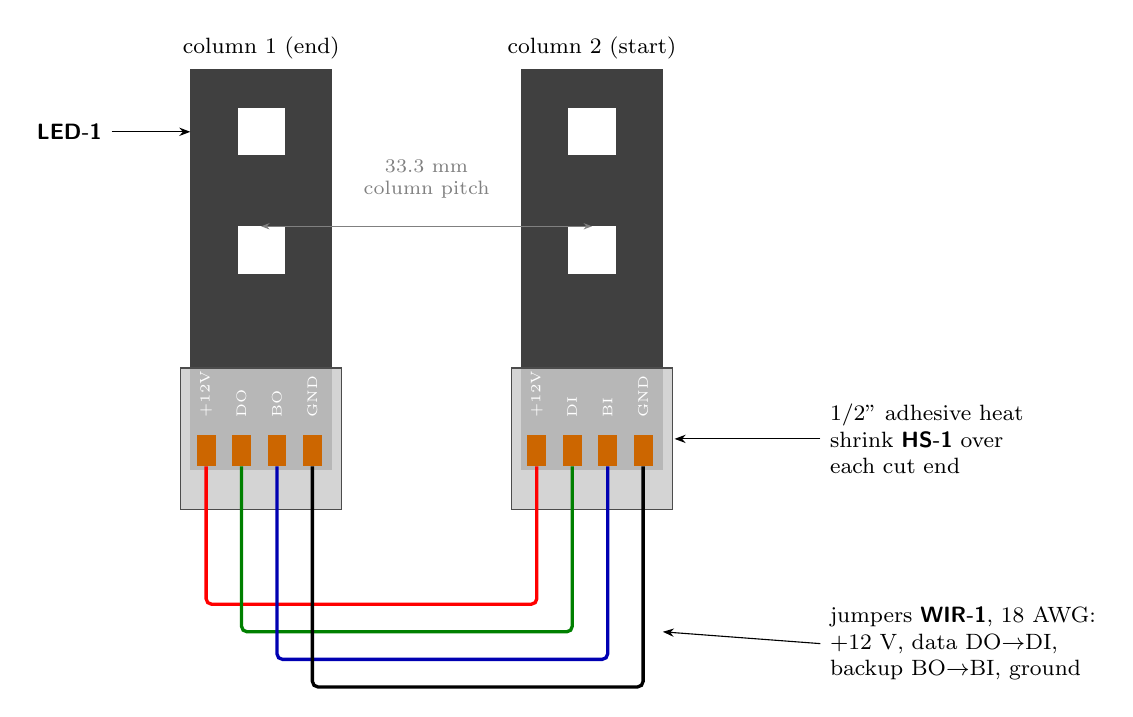
\begin{tikzpicture}[font=\footnotesize,
    callout/.style={-{Stealth[length=4pt]}, thin}]
  % strips: column 1 end (left, data arriving from above) and column 2 start (right, data leaving upward)
  \foreach \x/\lab in {0/{column 1 (end)}, 4.2/{column 2 (start)}} {
    \fill[black!75] (\x,0.9) rectangle (\x+1.8,6);
    \foreach \y in {4.9,3.4} { \fill[white] (\x+0.6,\y) rectangle (\x+1.2,\y+0.6); }
    \node[above] at (\x+0.9,6) {\lab};
    % heat shrink seal over the cut end
    \fill[gray!40, opacity=0.85] (\x-0.12,0.4) rectangle (\x+1.92,2.2);
    \draw[gray!60!black] (\x-0.12,0.4) rectangle (\x+1.92,2.2);
  }
  % pads at the cut ends (labels per side) and jumpers
  \foreach \i/\ll/\rl/\col in {0/{+12V}/{+12V}/red, 1/{DO}/{DI}/green!50!black, 2/{BO}/{BI}/blue!70!black, 3/{GND}/{GND}/black} {
    \pgfmathsetmacro{\px}{0.2+\i*0.45}
    \fill[orange!80!black] (\px-0.12,0.95) rectangle (\px+0.12,1.35);
    \fill[orange!80!black] (4.2+\px-0.12,0.95) rectangle (4.2+\px+0.12,1.35);
    \node[font=\tiny, white, rotate=90, anchor=west] at (\px,1.45) {\ll};
    \node[font=\tiny, white, rotate=90, anchor=west] at (4.2+\px,1.45) {\rl};
    \pgfmathsetmacro{\d}{-0.8-\i*0.35}
    \draw[\col, very thick, rounded corners=2pt] (\px,0.95) -- (\px,\d) -- (4.2+\px,\d) -- (4.2+\px,0.95);
  }
  \draw[callout] (8.0,-1.3) node[right, align=left] {jumpers \id{WIR-1}, 18 AWG:\\+12 V, data DO$\to$DI,\\backup BO$\to$BI, ground} -- (6.0,-1.15);
  \draw[callout] (8.0,1.3) node[right, align=left] {1/2'' adhesive heat\\shrink \id{HS-1} over\\each cut end} -- (6.15,1.3);
  \draw[callout] (-1.0,5.2) node[left, align=right] {\id{LED-1}} -- (0,5.2);
  \node[gray, font=\scriptsize, align=center] at (3.0,4.6) {33.3 mm\\column pitch};
  \draw[gray, {Stealth[length=3pt]}-{Stealth[length=3pt]}] (0.9,4.0) -- (5.1,4.0);
\end{tikzpicture}

  \caption{Corner joint (C1 shown).  Four 18~AWG jumpers \id{WIR-1}: \SI{12}{V}, data (DO to DI), backup data
    (BO to BI), ground.  Each cut end sealed with 1/2'' adhesive heat shrink \id{HS-1}.}
  \label{fig:corner}
\end{figure}

\section{Power fan-out}

Figure~\ref{fig:fanout} shows the power path; Figure~\ref{fig:runs} the layout along the top rail.
\begin{itemize}
  \item \textbf{Mains:} a plug-ended cord (\id{HD-3}) to a GFCI outdoor outlet, spliced to the supply's AC leads
    in a weatherproof splice (\id{HD-4}).  The house breaker protects the cord.
  \item \textbf{Supply} \id{PS-1}: HLG-600H-12B, \SI{12}{V} \SI{40}{A} \SI{480}{W}, IP67, fanless, universal input
    \SIrange{90}{305}{V} AC.  Its dimming wires are unused: capped and insulated (open means full output).
  \item \textbf{Links} (\id{HD-1}): the supply's output to the two fuse blocks' + studs and the two bus bars'
    studs; heavy enough for the supply's current limit, so nothing upstream of the fuses needs its own fuse.
  \item \textbf{Fuse blocks} \id{FB-1} (two, 8 circuits each) with one \SI{5}{A} ATO fuse \id{FU-1} per module:
    block A feeds M01--M07, block B M08--M14; one spare circuit each.
  \item \textbf{Ground bus bars} \id{BB-1} (two, 12 screws each): one per block.
  \item \textbf{Home runs:} one 18~AWG pair (\id{WIR-1}) per module, red from its fuse to the module's input plug
    power lead, black from there back to the bus bar; ring terminals \id{HD-2} at the blocks, soldered and
    heat-shrunk (\id{HS-2}) at the pigtail.  Runs are at most about \SI{1.5}{m}.
  \item \textbf{Protection by layers,} each guarding the wiring after it: the house breaker (cord); the supply's
    own current limit (links); a \SI{5}{A} fuse (each home run and module).
  \item \textbf{Rule:} switch off before plugging or unplugging a module (there are no bulk capacitors).
\end{itemize}

\begin{figure}[!htbp]
  \centering
  % Power fan-out: mains -> PS-1 -> links -> two fuse blocks (5 A per module) -> home runs (red) to the modules;
% returns (black) from the modules to two ground bus bars on the far side; data chain (dashed) between modules.
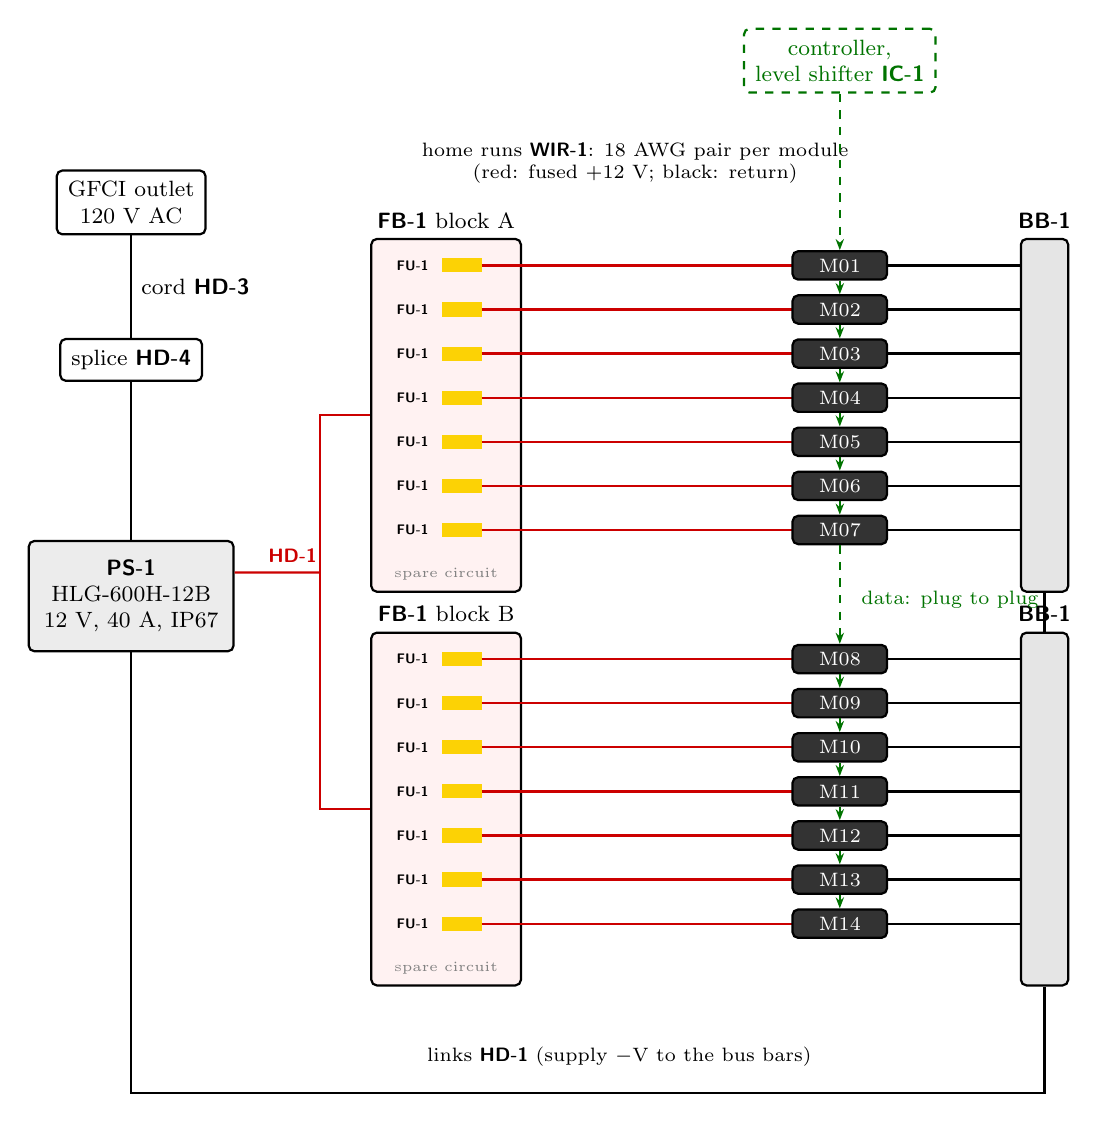
\begin{tikzpicture}[font=\footnotesize,
    box/.style={draw, thick, rounded corners=2pt, align=center, inner sep=4pt},
    mod/.style={draw, thick, rounded corners=2pt, font=\scriptsize, minimum width=1.2cm, minimum height=0.36cm,
                inner sep=1pt, fill=black!80, text=white},
    pwr/.style={thick, red!80!black},
    gnd/.style={thick, black},
    dat/.style={thick, dashed, green!45!black, -{Stealth[length=4pt]}}]
  \def\row{0.56}
  % mains and supply
  \node[box] (outlet) at (0,0.6) {GFCI outlet\\120 V AC};
  \node[box] (splice) at (0,-1.4) {splice \id{HD-4}};
  \node[box, minimum width=2.6cm, minimum height=1.4cm, fill=gray!15] (ps) at (0,-4.4) {\id{PS-1}\\HLG-600H-12B\\12 V, 40 A, IP67};
  \draw[thick] (outlet) -- node[right] {cord \id{HD-3}} (splice);
  \draw[thick] (splice) -- (ps);
  % two groups: block A (M01-M07) and block B (M08-M14)
  \foreach \blk/\ytop/\first in {A/0/1, B/-5.0/8} {
    \node[box, minimum width=1.9cm, minimum height={8*\row cm}, fill=red!5, anchor=north] (fb\blk) at (4.0,\ytop+0.15) {};
    \node[above] at (fb\blk.north) {\id{FB-1} block \blk};
    \node[box, minimum width=0.6cm, minimum height={8*\row cm}, fill=gray!20, anchor=north] (bb\blk) at (11.6,\ytop+0.15) {};
    \node[above] at (bb\blk.north) {\id{BB-1}};
    \foreach \j in {0,...,7} {
      \pgfmathsetmacro{\y}{\ytop - 0.2 - \j*\row}
      \pgfmathtruncatemacro{\m}{\first+\j}
      \ifnum\j<7
        \fill[yellow!70!orange] (3.95,\y-0.09) rectangle (4.45,\y+0.09);
        \node[font=\tiny, left] at (3.9,\y) {\id{FU-1}};
        \draw[pwr] (4.45,\y) -- (8.4,\y);
        \node[mod] (M\m) at (9.0,\y) {M\ifnum\m<10 0\fi\m};
        \draw[gnd] (9.6,\y) -- (11.3,\y);
      \else
        \node[font=\tiny, gray] at (4.0,\y) {spare circuit};
      \fi
    }
  }
  % links from the supply: + to both blocks, - to both bus bars
  \draw[pwr] (ps.east) ++(0,0.3) -- (2.4,-4.1) coordinate (r0);
  \draw[pwr] (r0) |- (fbA.west);
  \draw[pwr] (r0) |- (fbB.west);
  \node[red!80!black, font=\scriptsize, above] at (2.05,-4.1) {\id{HD-1}};
  \draw[gnd] (ps.south) -- ++(0,-5.6) -| (bbB.south);
  \draw[gnd] (bbB.north) -- (bbA.south);
  \node[font=\scriptsize, below] at (6.2,-10.0) {links \id{HD-1} (supply $-$V to the bus bars)};
  \node[font=\scriptsize, align=center] at (6.4,1.1) {home runs \id{WIR-1}: 18 AWG pair per module\\(red: fused +12 V; black: return)};
  % data chain: controller -> M01, then module to module through the plugs
  \node[box, dashed, green!45!black] (ic) at (9.0,2.4) {controller,\\level shifter \id{IC-1}};
  \draw[dat] (ic.south) -- (M1.north);
  \foreach \a/\b in {1/2,2/3,3/4,4/5,5/6,6/7,7/8,8/9,9/10,10/11,11/12,12/13,13/14} {
    \draw[dat] (M\a.south) -- (M\b.north);
  }
  \node[green!45!black, font=\scriptsize, align=left, right] at (9.15,-4.45) {data: plug to plug};
\end{tikzpicture}

  \caption{Power fan-out.  Mains cord \id{HD-3} and splice \id{HD-4} to the supply \id{PS-1}; links \id{HD-1} to
    two fuse blocks \id{FB-1} with \SI{5}{A} fuses \id{FU-1} and two ground bus bars \id{BB-1}; one 18~AWG home
    run \id{WIR-1} per module to its input plug.  Data (dashed) runs from the controller's level shifter
    \id{IC-1} through the modules' plugs.}
  \label{fig:fanout}
\end{figure}

\begin{figure}[!htbp]
  \centering
  % Top rail, front view: module inputs/outputs, data chain, home runs from the covered box behind the middle.
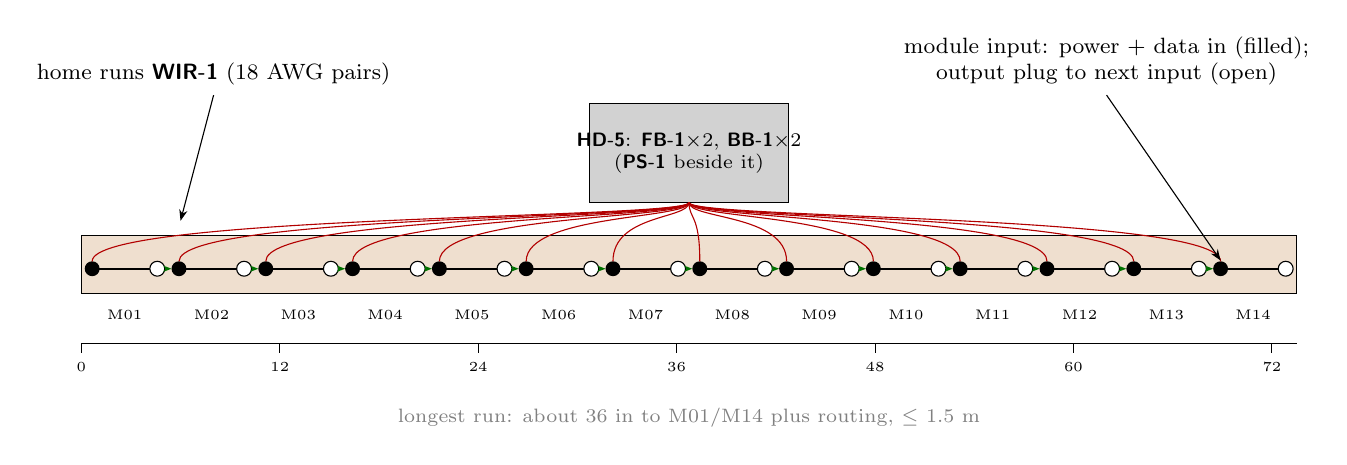
\begin{tikzpicture}[x=0.21cm, y=0.21cm, font=\footnotesize,
    callout/.style={-{Stealth[length=4pt]}, thin}]
  \def\p{1.3123}
  % top rail
  \fill[brown!25] (0,0) rectangle (73.5,3.5);
  \draw (0,0) rectangle (73.5,3.5);
  % covered box behind the middle of the top rail
  \fill[gray!35] (30.75,5.5) rectangle (42.75,11.5);
  \draw (30.75,5.5) rectangle (42.75,11.5);
  \node[font=\scriptsize, align=center] at (36.75,8.5) {\id{HD-5}: \id{FB-1}$\times$2, \id{BB-1}$\times$2\\(\id{PS-1} beside it)};
  % modules: input at column 4k (left), output at column 4k+3
  \foreach \k in {0,...,13} {
    \pgfmathsetmacro{\xi}{(4*\k+0.5)*\p}
    \pgfmathsetmacro{\xo}{(4*\k+3.5)*\p}
    \pgfmathtruncatemacro{\n}{\k+1}
    \draw[thick] (\xi,1.5) -- (\xo,1.5);
    \fill (\xi,1.5) circle (0.45);
    \fill[white] (\xo,1.5) circle (0.45); \draw (\xo,1.5) circle (0.45);
    \node[font=\tiny, below] at ({(\xi+\xo)/2},-0.4) {M\ifnum\n<10 0\fi\n};
    % home run from the box to the input
    \draw[red!70!black] (36.75,5.5) .. controls (36.75,4.5) and (\xi,4.8) .. (\xi,1.95);
  }
  % data chain: output of k to input of k+1 (adjacent)
  \foreach \k in {0,...,12} {
    \pgfmathsetmacro{\xo}{(4*\k+3.5)*\p}
    \pgfmathsetmacro{\xn}{(4*\k+4.5)*\p}
    \draw[green!45!black, thick, -{Stealth[length=3pt]}] (\xo+0.45,1.5) -- (\xn-0.45,1.5);
  }
  % scale
  \foreach \x in {0,12,24,36,48,60,72} { \draw (\x,-3.0) -- (\x,-3.6); \node[font=\tiny, below] at (\x,-3.6) {\x}; }
  \draw (0,-3.0) -- (73.5,-3.0);
  % callouts
  \draw[callout] (8,12) node[above, align=center] {home runs \id{WIR-1} (18 AWG pairs)} -- (6,4.4);
  \draw[callout] (62,12) node[above, align=center] {module input: power + data in (filled);\\output plug to next input (open)} -- ({(52+0.5)*\p},2.0);
  \node[font=\scriptsize, align=center, gray] at (36.75,-7.5) {longest run: about 36 in to M01/M14 plus routing, $\le$ 1.5 m};
\end{tikzpicture}

  \caption{Top rail, seen from the front: module inputs (filled) and outputs (open), the plug-to-plug data chain,
    and the home runs \id{WIR-1} from the covered box \id{HD-5} (fuse blocks \id{FB-1}, bus bars \id{BB-1}) behind
    the middle of the top rail.  Horizontal scale in inches from the LED area's left edge.}
  \label{fig:runs}
\end{figure}

\section{Numbers}
\label{sec:numbers}

BTF-LIGHTING rates a reel at \SI{12}{V} \SI{3}{A} (\SI{36}{W}) at full white; a module uses 148 of its 150 LEDs.

\begin{center}
\begin{tabular}{@{}lrrrr@{}}
  \toprule
  case & per module & panel at \SI{12}{V} & panel power & supply load \\
  \midrule
  full white, 100\,\%     & \SI{3.0}{A} & \SI{42}{A} & \SI{504}{W} & 105\,\% (over) \\
  75\,\% cap              & \SI{2.2}{A} & \SI{32}{A} & \SI{378}{W} & 79\,\% \\
  \textbf{50\,\% cap (design)} & \SI{1.5}{A} & \SI{21}{A} & \SI{252}{W} & 52\,\% \\
  typical scene, 50\,\%   & $<\SI{0.5}{A}$ & $<\SI{6}{A}$ & $<\SI{70}{W}$ & $<15\,\%$ \\
  \bottomrule
\end{tabular}
\end{center}

\begin{itemize}
  \item \textbf{At the wall:} about \SI{280}{W} at the 50\,\% cap, about \SI{2.5}{A} at \SI{120}{V}.
  \item \textbf{Fuses:} \SI{5}{A} is the next standard size above 125\,\% of \SI{3}{A}; it never blows in normal
    use and protects 18~AWG.
  \item \textbf{Home-run drop:} \SI{1.5}{m} of 18~AWG out and back is about \SI{0.06}{\ohm}:
    \SI{0.1}{V} at \SI{1.5}{A}, \SI{0.2}{V} at \SI{3}{A}.
  \item \textbf{Along a module} (fed at one end): about \SI{1}{V} at the 50\,\% cap, about \SI{2}{V} at full
    white (estimate); WS2815 LEDs are constant-current and hold their color to about \SI{10}{V}.  To be measured
    on the pilot.
  \item \textbf{Data:} one chain of 2072 pixels takes about \SI{62}{ms} per frame (about 16 frames per second);
    splitting into more chains, or one line per module from the Zynq, is a matter of unplugging joints.
\end{itemize}

\section{Pilot}
\label{sec:pilot}

One reel, ordered 2026-10-19 (Amazon order~1).  Before cutting: light the whole reel from a lab \SI{12}{V}
supply with current limiting (start at \SI{1}{A}; about \SI{3.5}{A} for full white), check every LED and the
color order, and measure the far end.  Then: measure the pitch over 37 LEDs, fit a clip, cut and solder the
three corners, seal, mount on two slats, and repeat the test, including the voltage at the far end at the
50\,\% cap.

\section{Bill of materials}
\label{sec:bom}

Prices as read 2026-10-18/19, before shipping and tax.  Order: P = Amazon pilot (placed), A2 = Amazon order~2
(after the pilot), DK = DigiKey order v1, HD = Home Depot (when laying out), OH = on hand.
Links: \url{https://www.amazon.com/dp/<ASIN>}.

\begin{center}
\small
\begin{tabularx}{\linewidth}{@{}l>{\raggedright\arraybackslash}Xrlll r@{}}
  \toprule
  ID & item & qty & order & source & part / ASIN & total \\
  \midrule
  \id{LED-1} & BTF-LIGHTING WS2815, \SI{12}{V}, \SI{5}{m}, 150 LEDs, IP65, gold wire, backup data & 1+14 & P, A2 & Amazon & B07LG54F4W & \$449.85 \\
  \id{MNT-1} & BTF-LIGHTING transparent strip clips, 12~mm, 100 + screws per pack & 2 & P & Amazon & B0DM8VL3R4 & \$27.98 \\
  \id{WIR-1} & TUOFENG 18~AWG silicone wire, tinned copper, 50~ft red + 50~ft black per pack & 1+1 & P, A2 & Amazon & B07FMWNF3J & \$33.98 \\
  \id{HS-1} & XHF heat shrink 1/2'', 3:1 adhesive-lined, black, 10~ft & 1 & P & Amazon & B0919K23RX & \$6.29 \\
  \id{HS-2} & XHF heat shrink 3/16'', 3:1 adhesive-lined, black, 20~ft & 1 & P & Amazon & B0919F4YFZ & \$7.99 \\
  \id{IC-1} & SN74AHCT125N, DIP-14, generic 10-pack (pilot, spares) & 1 & P & Amazon & B08R6BCSYC & \$7.99 \\
  \id{IC-2} & SN74AHCT125N, Texas Instruments (installation) & 5 & DK & DigiKey & 296-4655-5-ND & \$5.00 \\
  \id{PS-1} & Mean Well HLG-600H-12B, \SI{12}{V} \SI{40}{A} \SI{480}{W}, IP67 & 1 & DK & DigiKey & 1866-2567-ND & \$209.00 \\
  \id{FB-1} & Fuse block, 8 circuits, ATO/ATC, \#8-32 outputs, \#10-32 stud, cover & 2 & A2 & Amazon & B0F7P88MZ2 & \$47.98 \\
  \id{BB-1} & RVBOATPAT ground bus bar, $12\times$\#8 screws, 1/4'' stud, cover & 2 & A2 & Amazon & B0F6SC5C3Q & \$19.96 \\
  \id{FU-1} & Littelfuse 0287005.PXCN, \SI{5}{A} ATO fuse & 20 & DK & DigiKey & F4197-ND & \$6.66 \\
  \midrule
  \id{FR-1} & 2x6, 8~ft (two cut 77'', two 56'') & 4 & OH & lumber & & -- \\
  \id{FR-2} & 2x4, 8~ft (two rails, about 74'') & 2 & OH & lumber & & -- \\
  \id{FR-3} & 1x2, 8~ft (slats, 56'' each; 28 + 2 spare) & 30 & OH & lumber & & -- \\
  \midrule
  \id{HD-1} & Links, supply to blocks and bus bars, 12--10~AWG, ring terminals (\#10, 1/4'') & -- & HD & Home Depot & & -- \\
  \id{HD-2} & Ring terminals, \#8, 22--16~AWG, heat-shrink sealed (about 50) & -- & HD & Home Depot & & -- \\
  \id{HD-3} & Plug-ended outdoor cord, 3 conductors (or one on hand) & 1 & HD & Home Depot & & -- \\
  \id{HD-4} & Weatherproof splice for the supply's AC leads & 1 & HD & Home Depot & & -- \\
  \id{HD-5} & Covered box for fuse blocks and bus bars & 1 & HD & Home Depot & & -- \\
  \bottomrule
\end{tabularx}
\end{center}

\noindent Totals: Amazon pilot \$97.23 (placed); Amazon order~2 \$504.79; DigiKey v1 \$220.66; together \$822.68,
plus Home Depot items.

\end{document}
